\documentclass{article}\usepackage[]{graphicx}\usepackage[]{color}
%% maxwidth is the original width if it is less than linewidth
%% otherwise use linewidth (to make sure the graphics do not exceed the margin)
\makeatletter
\def\maxwidth{ %
  \ifdim\Gin@nat@width>\linewidth
    \linewidth
  \else
    \Gin@nat@width
  \fi
}
\makeatother

\definecolor{fgcolor}{rgb}{0.345, 0.345, 0.345}
\newcommand{\hlnum}[1]{\textcolor[rgb]{0.686,0.059,0.569}{#1}}%
\newcommand{\hlstr}[1]{\textcolor[rgb]{0.192,0.494,0.8}{#1}}%
\newcommand{\hlcom}[1]{\textcolor[rgb]{0.678,0.584,0.686}{\textit{#1}}}%
\newcommand{\hlopt}[1]{\textcolor[rgb]{0,0,0}{#1}}%
\newcommand{\hlstd}[1]{\textcolor[rgb]{0.345,0.345,0.345}{#1}}%
\newcommand{\hlkwa}[1]{\textcolor[rgb]{0.161,0.373,0.58}{\textbf{#1}}}%
\newcommand{\hlkwb}[1]{\textcolor[rgb]{0.69,0.353,0.396}{#1}}%
\newcommand{\hlkwc}[1]{\textcolor[rgb]{0.333,0.667,0.333}{#1}}%
\newcommand{\hlkwd}[1]{\textcolor[rgb]{0.737,0.353,0.396}{\textbf{#1}}}%
\let\hlipl\hlkwb

\usepackage{framed}
\makeatletter
\newenvironment{kframe}{%
 \def\at@end@of@kframe{}%
 \ifinner\ifhmode%
  \def\at@end@of@kframe{\end{minipage}}%
  \begin{minipage}{\columnwidth}%
 \fi\fi%
 \def\FrameCommand##1{\hskip\@totalleftmargin \hskip-\fboxsep
 \colorbox{shadecolor}{##1}\hskip-\fboxsep
     % There is no \\@totalrightmargin, so:
     \hskip-\linewidth \hskip-\@totalleftmargin \hskip\columnwidth}%
 \MakeFramed {\advance\hsize-\width
   \@totalleftmargin\z@ \linewidth\hsize
   \@setminipage}}%
 {\par\unskip\endMakeFramed%
 \at@end@of@kframe}
\makeatother

\definecolor{shadecolor}{rgb}{.97, .97, .97}
\definecolor{messagecolor}{rgb}{0, 0, 0}
\definecolor{warningcolor}{rgb}{1, 0, 1}
\definecolor{errorcolor}{rgb}{1, 0, 0}
\newenvironment{knitrout}{}{} % an empty environment to be redefined in TeX

\usepackage{alltt}
\usepackage[sc]{mathpazo}
\usepackage[T1]{fontenc}
\usepackage{geometry}
\geometry{verbose,tmargin=2.5cm,bmargin=2.5cm,lmargin=2.5cm,rmargin=2.5cm}
\setcounter{secnumdepth}{2}
\setcounter{tocdepth}{2}
\usepackage{url}
\usepackage[unicode=true,pdfusetitle,
 bookmarks=true,bookmarksnumbered=true,bookmarksopen=true,bookmarksopenlevel=2,
 breaklinks=false,pdfborder={0 0 1},backref=false,colorlinks=false,hidelinks]
 {hyperref}
\hypersetup{
 pdfstartview={XYZ null null 1}}
\usepackage{breakurl}
\IfFileExists{upquote.sty}{\usepackage{upquote}}{}
\begin{document}



\title{Image analysis in R}
\author{Tommaso Leonardi, tl344@ebi.ac.uk}
\date{November 24th, 2016}
\maketitle
\tableofcontents
\section{Loading an image}
For this tutorial we are going to need some external libraries, which can be loaded with:
\begin{knitrout}
\definecolor{shadecolor}{rgb}{0.969, 0.969, 0.969}\color{fgcolor}\begin{kframe}
\begin{alltt}
\hlkwd{library}\hlstd{(}\hlstr{"EBImage"}\hlstd{)}
\hlkwd{library}\hlstd{(}\hlstr{"tiff"}\hlstd{)}
\hlkwd{library}\hlstd{(}\hlstr{"ggplot2"}\hlstd{)}
\end{alltt}
\end{kframe}
\end{knitrout}

We can now load the image that we want to analyse:
\begin{knitrout}
\definecolor{shadecolor}{rgb}{0.969, 0.969, 0.969}\color{fgcolor}\begin{kframe}
\begin{alltt}
\hlstd{tif_files} \hlkwb{<-} \hlkwd{as.Image}\hlstd{(}\hlkwd{readTIFF}\hlstd{(}\hlstr{"astrocytes.tiff"}\hlstd{))}
\hlkwd{colorMode}\hlstd{(tif_files)} \hlkwb{<-} \hlstr{"color"}
\hlstd{nuc} \hlkwb{<-} \hlkwd{t}\hlstd{(tif_files[,,}\hlnum{1}\hlstd{])}
\hlstd{cel} \hlkwb{<-} \hlkwd{t}\hlstd{(tif_files[,,}\hlnum{3}\hlstd{])}
\hlstd{img} \hlkwb{=} \hlkwd{rgbImage}\hlstd{(}\hlkwc{green}\hlstd{=cel,} \hlkwc{blue}\hlstd{=nuc)}
\hlkwd{display}\hlstd{(img,} \hlkwc{method}\hlstd{=}\hlstr{"raster"}\hlstd{)}
\end{alltt}
\end{kframe}\begin{figure}

{\centering 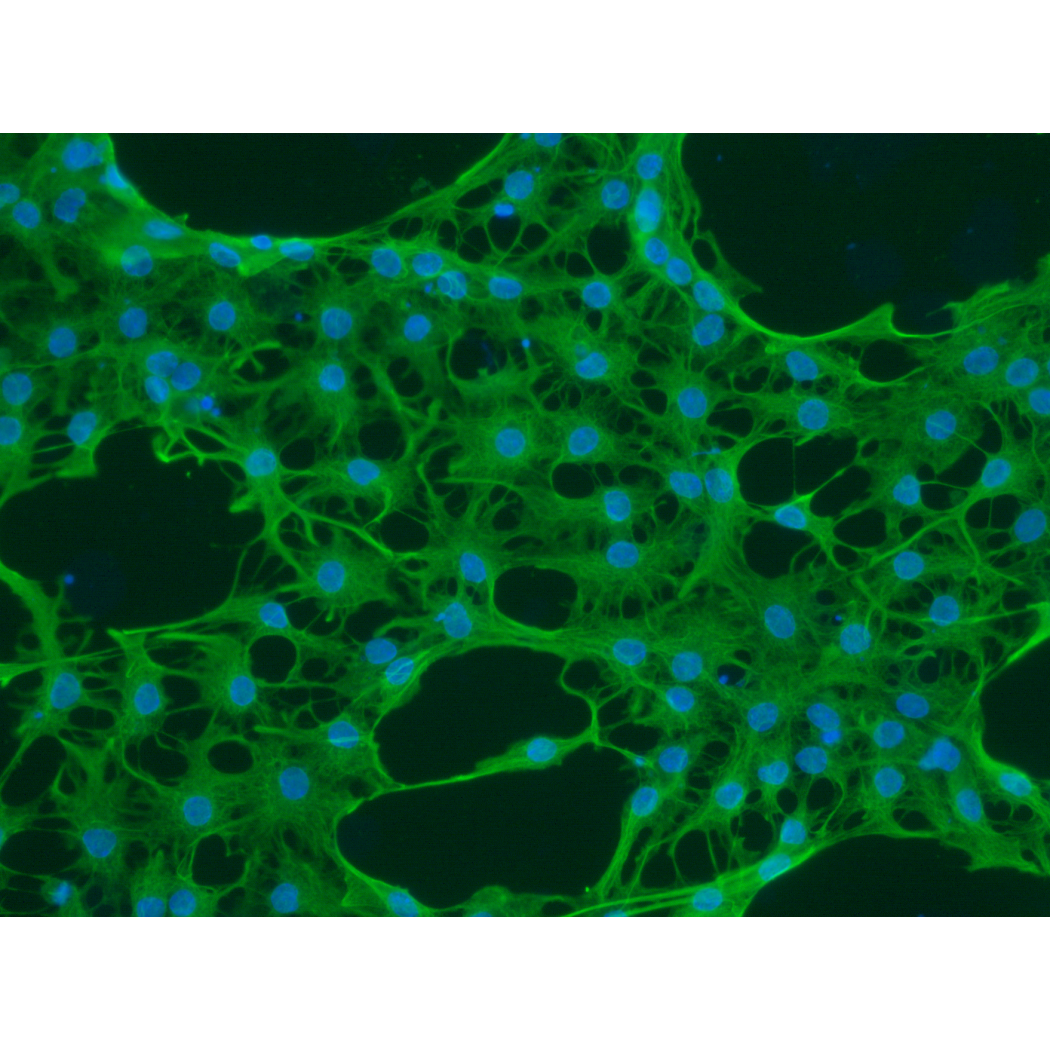
\includegraphics[width=\maxwidth]{knit_figure/figfull_image-1} 

}

\caption[The starting image that we want to analyse]{The starting image that we want to analyse}\label{fig:full.image}
\end{figure}


\end{knitrout}
The nuc object now contains the channel with the DAPI staining, while the cel object contains the channel with the Vimentin staining.
The last two commands combine the two channels in a single RGB image and display it (Figure \ref{fig:full.image}). From this image, we want to determine:
\begin{enumerate}
  \item The number of cells
  \item The average signal intensity per cell
  \item The distribution of the areas of the cells
\end{enumerate}

\section{Segmenting nuclei}
\begin{knitrout}
\definecolor{shadecolor}{rgb}{0.969, 0.969, 0.969}\color{fgcolor}\begin{figure}

{\centering 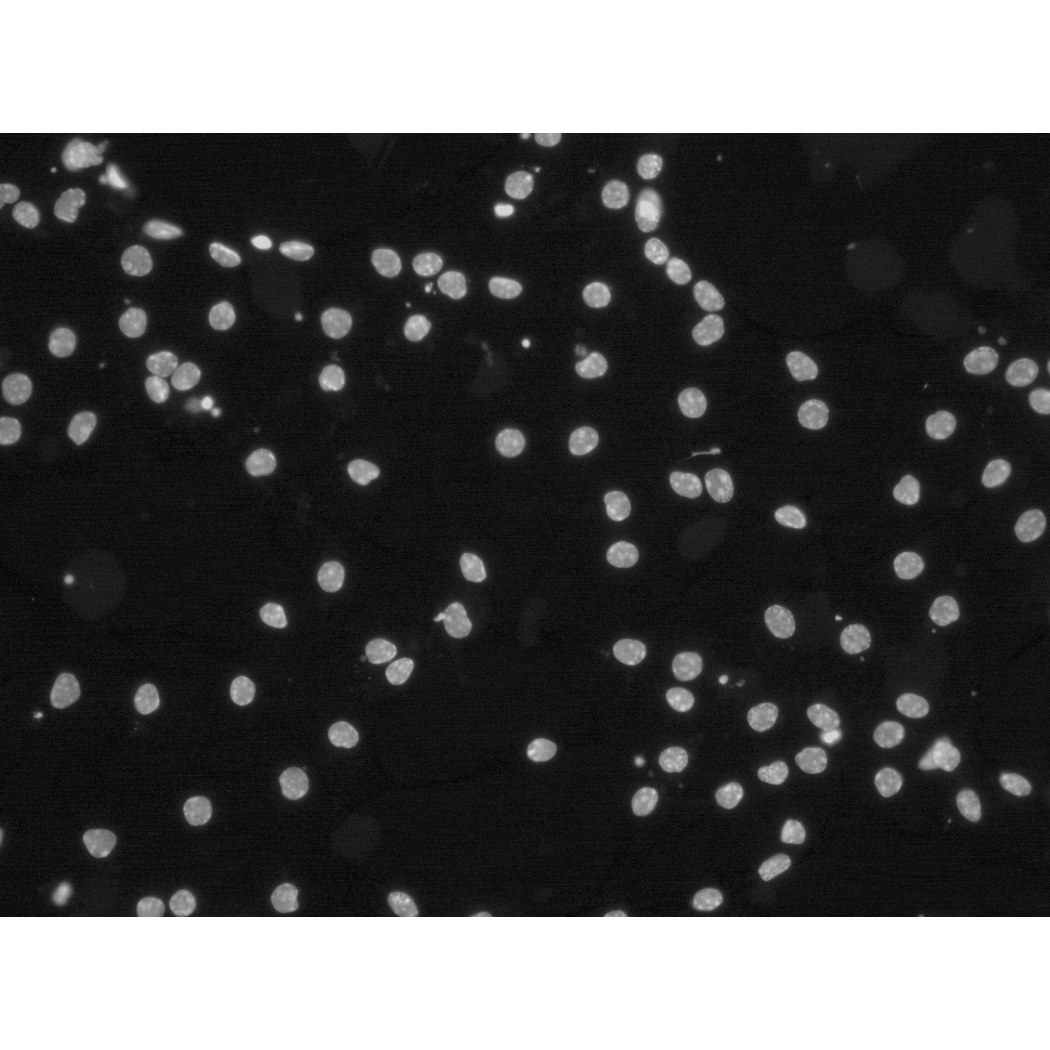
\includegraphics[width=200px]{knit_figure/figdapi-1} 

}

\caption[Object nuc (i.e., DAPI channel)]{Object nuc (i.e., DAPI channel)}\label{fig:dapi}
\end{figure}


\end{knitrout}
The first step is to identify the nuclei based on the DAPI staining (Figure \ref{fig:dapi}).
The simplest approach is to just apply a threshold on the image:
\begin{knitrout}
\definecolor{shadecolor}{rgb}{0.969, 0.969, 0.969}\color{fgcolor}\begin{kframe}
\begin{alltt}
\hlstd{nmask} \hlkwb{<-} \hlstd{nuc} \hlopt{>} \hlnum{0.3}
\end{alltt}
\end{kframe}\begin{figure}

{\centering 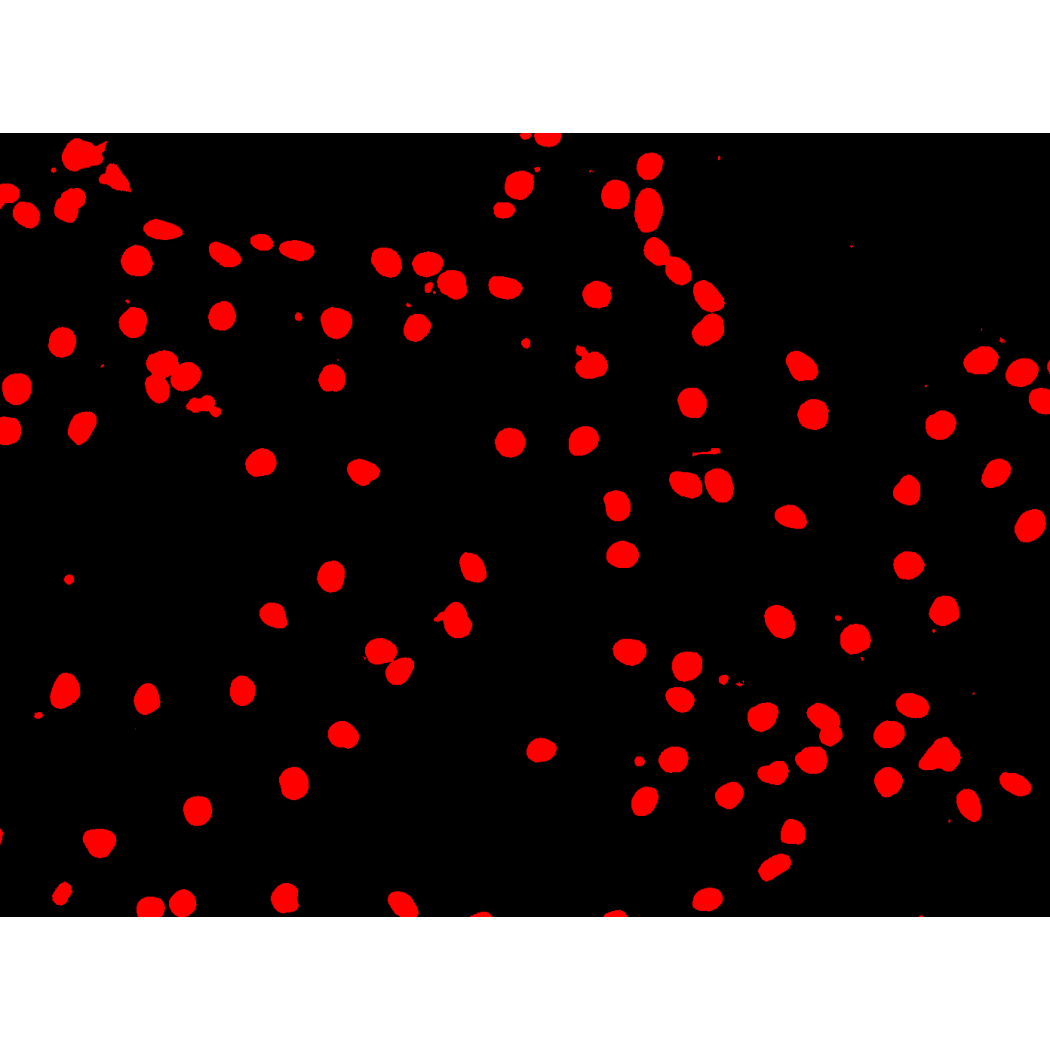
\includegraphics[width=200px]{knit_figure/figsimp_thr-1} 

}

\caption[Simple thresholding]{Simple thresholding}\label{fig:simp.thr}
\end{figure}


\end{knitrout}
Which would generate a binary image as in Figure \ref{fig:simp.thr}.
However, the EBImage package provides the thresh function, which is slightly more elaborate (type '?thresh' for more info) and gives better results.

\begin{knitrout}
\definecolor{shadecolor}{rgb}{0.969, 0.969, 0.969}\color{fgcolor}\begin{kframe}
\begin{alltt}
\hlstd{nmask} \hlkwb{=} \hlkwd{thresh}\hlstd{(nuc,} \hlkwc{w}\hlstd{=}\hlnum{35}\hlstd{,} \hlkwc{h}\hlstd{=}\hlnum{35}\hlstd{,} \hlkwc{offset}\hlstd{=}\hlnum{0.15}\hlstd{)}
\hlkwd{display}\hlstd{(nmask,} \hlkwc{method}\hlstd{=}\hlstr{"raster"}\hlstd{)}
\end{alltt}
\end{kframe}\begin{figure}

{\centering 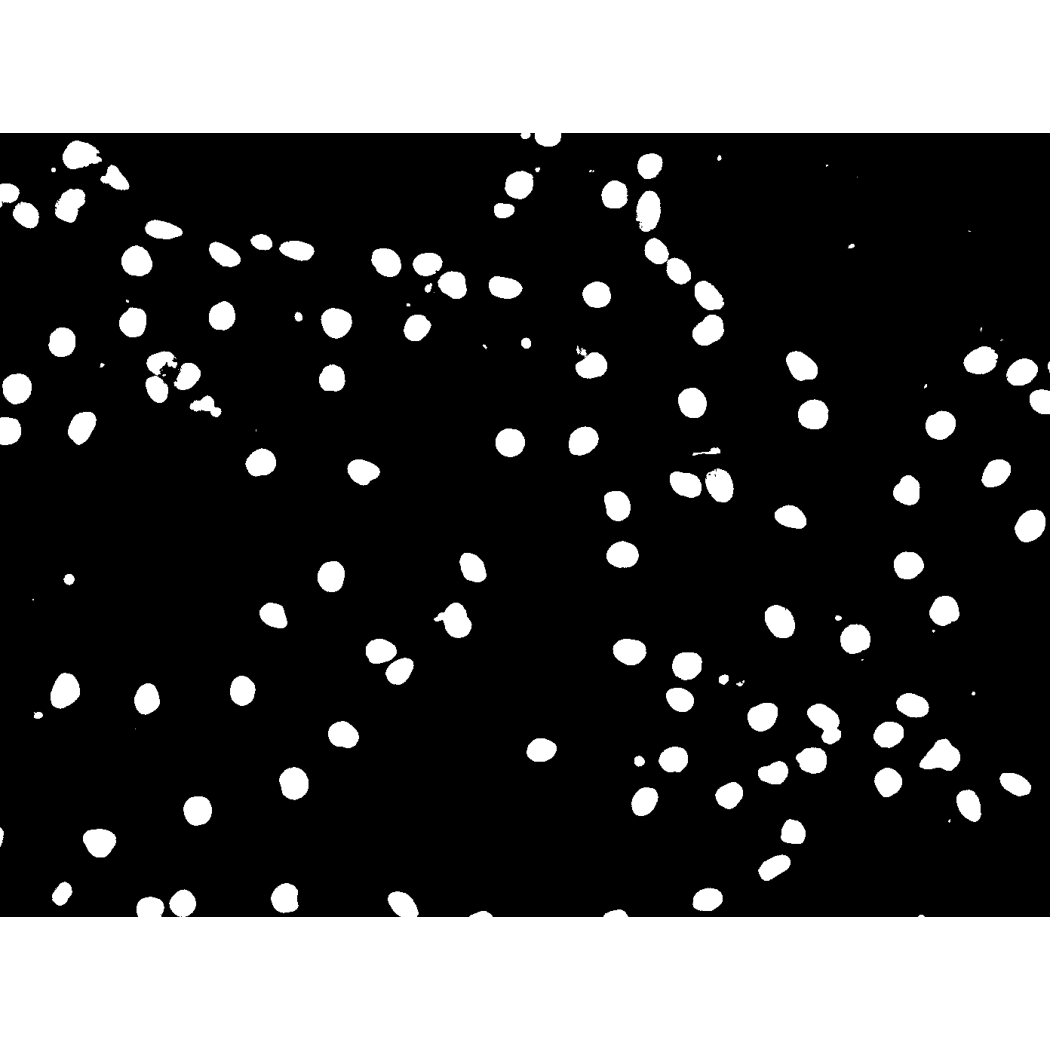
\includegraphics[width=200px]{knit_figure/figthr-1} 

}

\caption[Nuclei thresholded using the thresh() function in EBImage]{Nuclei thresholded using the thresh() function in EBImage}\label{fig:thr}
\end{figure}


\end{knitrout}
The thresh function compares the image (nuc) to its filtered (smoothed) version. The w and h parameters in thresh() define the width and the height of the filtering window, while offset specifies the required difference in intensity between the original and filtered versions. The result is displayed in Figure \ref{fig:thr}.


\begin{knitrout}
\definecolor{shadecolor}{rgb}{0.969, 0.969, 0.969}\color{fgcolor}\begin{kframe}
\begin{alltt}
\hlstd{nmask} \hlkwb{=} \hlkwd{opening}\hlstd{(nmask,} \hlkwd{makeBrush}\hlstd{(}\hlnum{15}\hlstd{,} \hlkwc{shape}\hlstd{=}\hlstr{"disc"}\hlstd{))}
\hlstd{nmask} \hlkwb{=} \hlkwd{fillHull}\hlstd{(nmask)}
\hlstd{nmask} \hlkwb{=} \hlkwd{bwlabel}\hlstd{(nmask)}
\hlkwd{display}\hlstd{(nmask,} \hlkwc{method}\hlstd{=}\hlstr{"raster"}\hlstd{)}
\end{alltt}
\end{kframe}\begin{figure}

{\centering 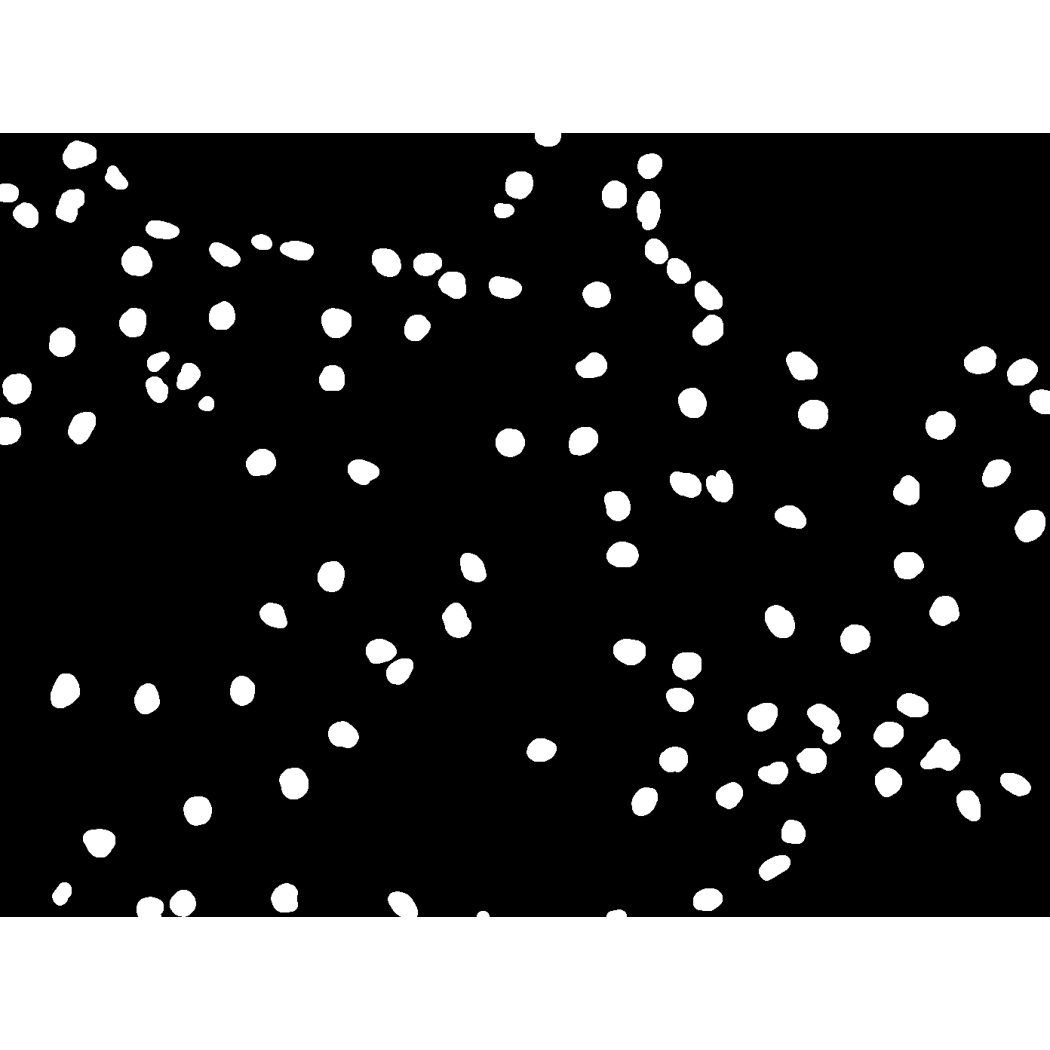
\includegraphics[width=200px]{knit_figure/figopening-1} 

}

\caption[Segmented nuclei after opening() and fillHull()]{Segmented nuclei after opening() and fillHull()}\label{fig:opening}
\end{figure}


\end{knitrout}
The opening() function performs an erosion followed by a dilation\footnotemark[1] with a filter of size 15. As you can see in Figure \ref{fig:opening}, the effect if that we get rid of several small objects that are clearly noise.
The last two lines perform to simple actions: fillHull fills the holes inside the segmented nuclei (i.e. sets to 1 all the 0s that are surrounded by 1s), while bwlabel assigns a label to each nucleus.

\footnotetext[1]{In very simple terms, erode() removes a bit from the border of every object, while dilate adds a bit to the border of every object. The trick here is that for small objects, the erosion completely removes them.}

Finally, we can annotate the original image with the position of the segmented nuclei (Figure \ref{fig:nucgray}):
\begin{knitrout}
\definecolor{shadecolor}{rgb}{0.969, 0.969, 0.969}\color{fgcolor}\begin{kframe}
\begin{alltt}
\hlkwd{colorMode}\hlstd{(nmask)} \hlkwb{<-} \hlstr{"Grayscale"}
\hlstd{nucgray} \hlkwb{=} \hlkwd{channel}\hlstd{(nuc,} \hlstr{"rgb"}\hlstd{)}
\hlstd{nucgray} \hlkwb{=} \hlkwd{paintObjects}\hlstd{(nmask, nucgray,} \hlkwc{col}\hlstd{=}\hlstr{"#ff00ff"}\hlstd{)}
\hlkwd{display}\hlstd{(nucgray,} \hlkwc{method}\hlstd{=}\hlstr{"raster"}\hlstd{)}
\end{alltt}
\end{kframe}\begin{figure}

{\centering 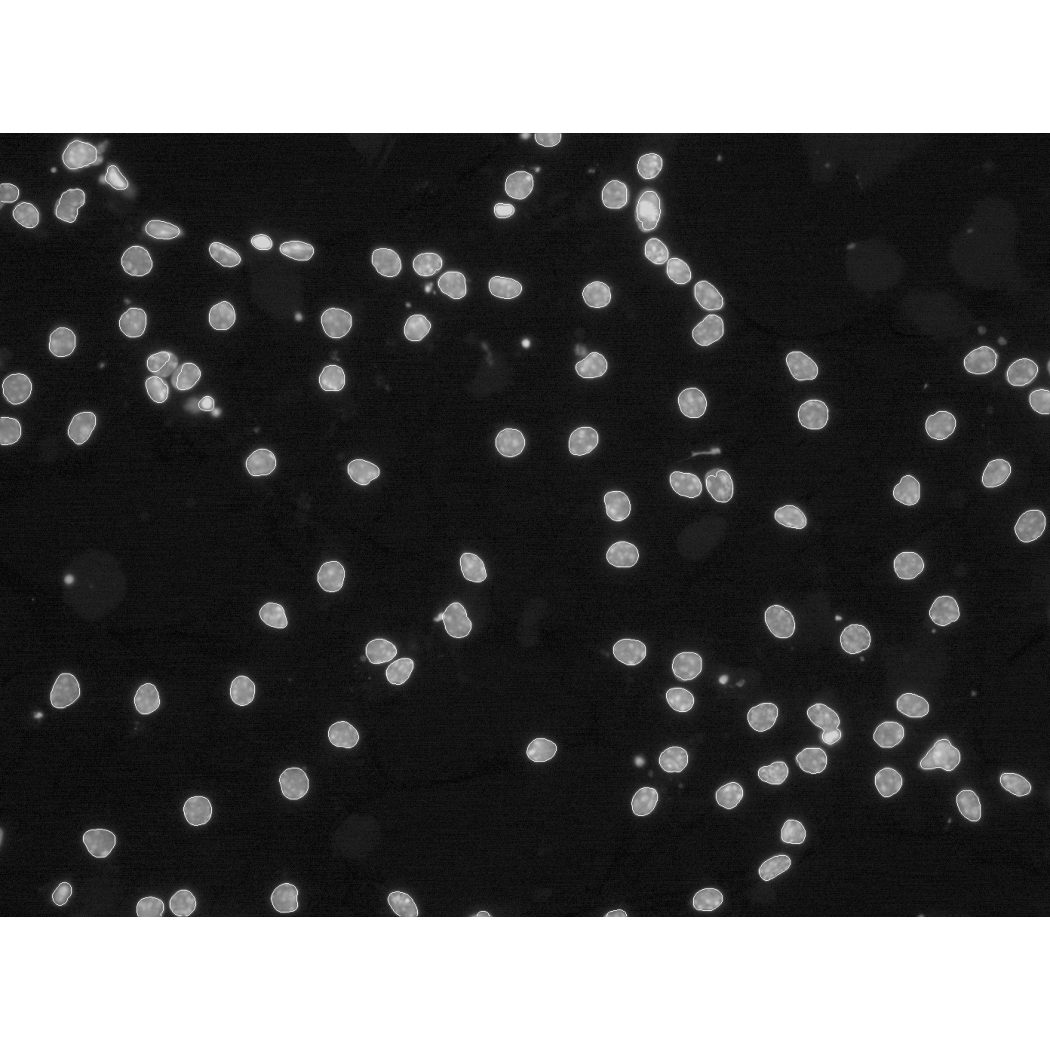
\includegraphics[width=300px]{knit_figure/fignucgray-1} 

}

\caption[Final image showing segmented nuclei]{Final image showing segmented nuclei}\label{fig:nucgray}
\end{figure}


\end{knitrout}

\section{Segmenting the cell bodies}
We first make a mask based on the intensity of the Vimentin channell:
\begin{knitrout}
\definecolor{shadecolor}{rgb}{0.969, 0.969, 0.969}\color{fgcolor}\begin{kframe}
\begin{alltt}
\hlstd{ctmask} \hlkwb{=} \hlkwd{opening}\hlstd{(cel}\hlopt{>}\hlnum{0.3}\hlstd{,} \hlkwd{makeBrush}\hlstd{(}\hlnum{5}\hlstd{,} \hlkwc{shape}\hlstd{=}\hlstr{"disc"}\hlstd{))}
\end{alltt}
\end{kframe}
\end{knitrout}
And then using the propagate() function we determine the object boundaries in the cel image based previously identified seeds (i.e. the segmented nuclei). The result is displayed in Figure \ref{fig:cmask}.
\begin{knitrout}
\definecolor{shadecolor}{rgb}{0.969, 0.969, 0.969}\color{fgcolor}\begin{kframe}
\begin{alltt}
\hlstd{cmask} \hlkwb{=} \hlkwd{propagate}\hlstd{(cel,} \hlkwc{seeds}\hlstd{=nmask,} \hlkwc{mask}\hlstd{=ctmask,} \hlkwc{lambda}\hlstd{=}\hlnum{1e-1}\hlstd{)}
\hlstd{cmask} \hlkwb{=} \hlkwd{fillHull}\hlstd{(cmask)}
\hlkwd{display}\hlstd{(cmask,} \hlkwc{method}\hlstd{=}\hlstr{"raster"}\hlstd{)}
\end{alltt}
\end{kframe}\begin{figure}

{\centering 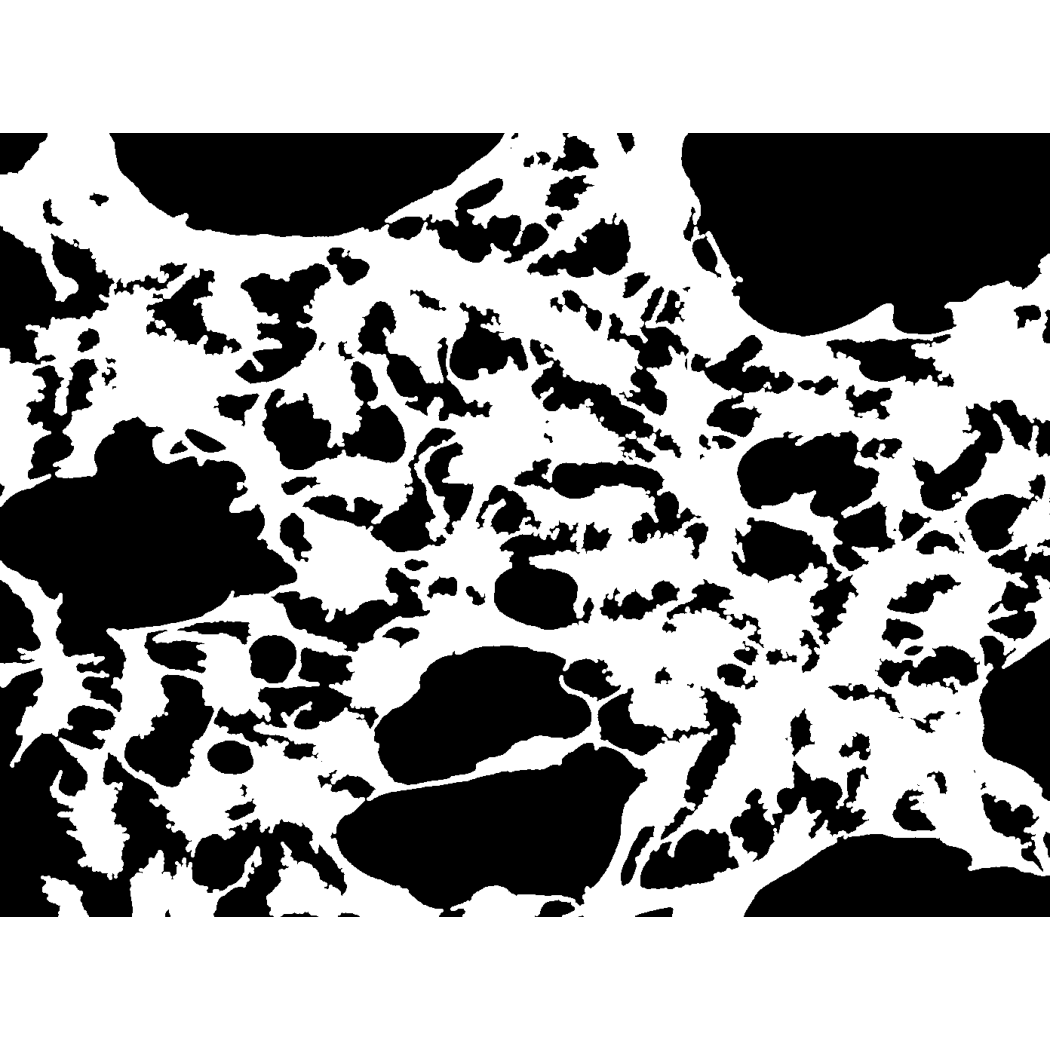
\includegraphics[width=200px]{knit_figure/figcmask-1} 

}

\caption[Segmented cell bodies]{Segmented cell bodies}\label{fig:cmask}
\end{figure}


\end{knitrout}
Finally, we can combine our segmented nuclei and cell bodies in a single image (Figure \ref{fig:res}):
\begin{knitrout}
\definecolor{shadecolor}{rgb}{0.969, 0.969, 0.969}\color{fgcolor}\begin{kframe}
\begin{alltt}
\hlkwd{colorMode}\hlstd{(cmask)} \hlkwb{<-} \hlstr{"Grayscale"}
\hlstd{res} \hlkwb{=} \hlkwd{paintObjects}\hlstd{(cmask, img,} \hlkwc{col}\hlstd{=}\hlstr{"#FF0000"}\hlstd{)}
\hlstd{res} \hlkwb{=} \hlkwd{paintObjects}\hlstd{(nmask, res,} \hlkwc{col}\hlstd{=}\hlstr{"#ffff00"}\hlstd{)}
\hlkwd{display}\hlstd{(res,} \hlkwc{method}\hlstd{=}\hlstr{"raster"}\hlstd{)}
\end{alltt}
\end{kframe}\begin{figure}

{\centering 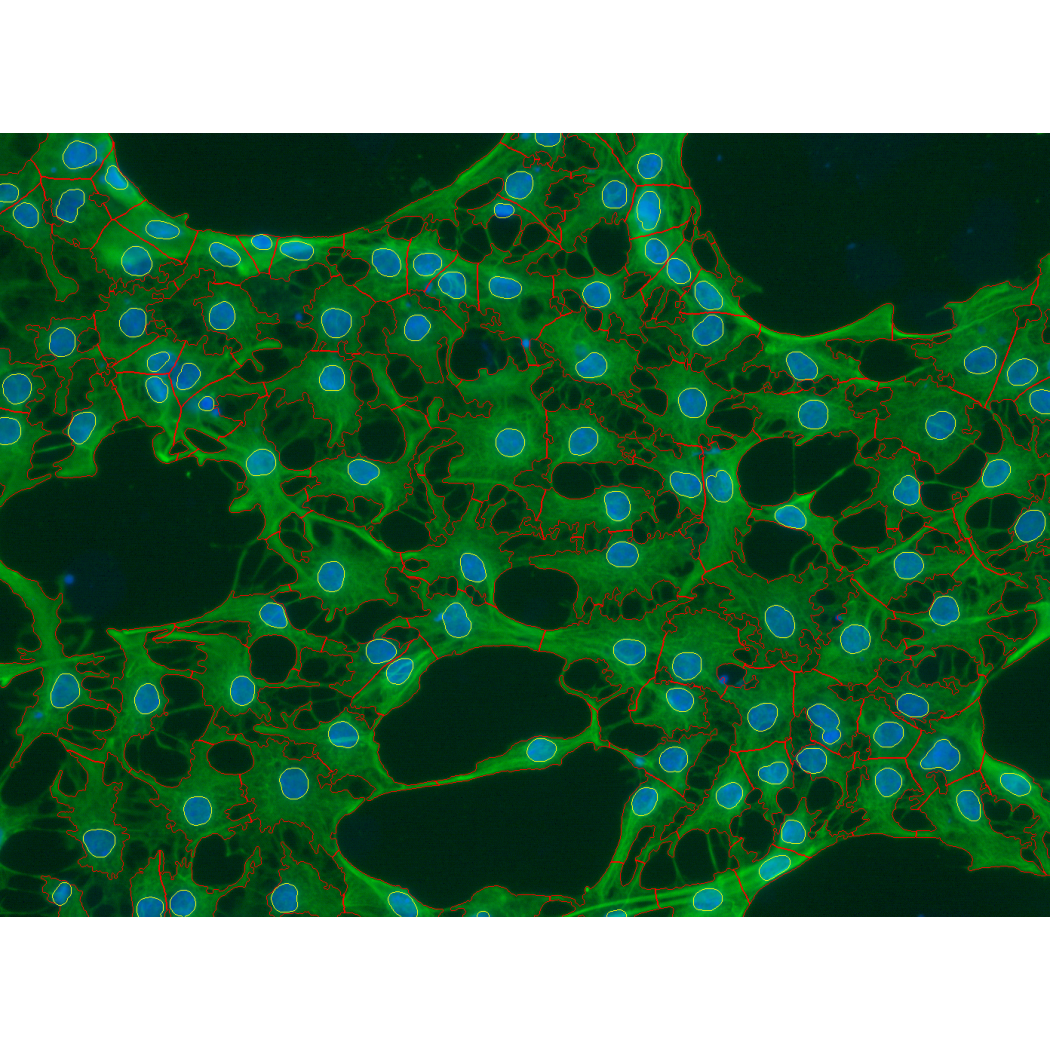
\includegraphics[width=400px]{knit_figure/figres-1} 

}

\caption[Segmented cell bodies]{Segmented cell bodies}\label{fig:res}
\end{figure}


\end{knitrout}

\section{Computing features}
Now that we know the boundaries of each cell we can easily calculate features such as cell size, mean signal intensity, etc...
This is easily done using the computeFeatures() function in EBImage. This function comes in three flavours: one to calculate intensities, one to calculate shape and one to calculate moment (i.e. position related things)
Let's compute the features and combine the interesting ones in a single dataframe:
\begin{knitrout}
\definecolor{shadecolor}{rgb}{0.969, 0.969, 0.969}\color{fgcolor}\begin{kframe}
\begin{alltt}
\hlstd{basic} \hlkwb{<-} \hlkwd{computeFeatures.basic}\hlstd{(cmask, cel)}
\hlstd{shape} \hlkwb{<-} \hlkwd{computeFeatures.shape}\hlstd{(cmask)}
\hlstd{moment} \hlkwb{<-} \hlkwd{computeFeatures.moment}\hlstd{(cmask)}
\hlstd{all_features} \hlkwb{<-} \hlkwd{as.data.frame}\hlstd{(}\hlkwd{cbind}\hlstd{(basic, shape, moment))}
\hlstd{all_features} \hlkwb{<-} \hlstd{all_features[,}\hlkwd{c}\hlstd{(}\hlnum{1}\hlstd{,}\hlnum{9}\hlstd{,}\hlnum{16}\hlstd{,}\hlnum{17}\hlstd{)]}
\hlkwd{head}\hlstd{(all_features)}
\end{alltt}
\begin{verbatim}
##      b.mean s.area     m.cy m.majoraxis
## 1 0.4047817   2318 16.16307    91.03620
## 2 0.4325038   5364 29.72185   107.81047
## 3 0.4563452   5784 34.00450   114.34311
## 4 0.4895764   3196 72.95494    87.78619
## 5 0.4185337  10045 74.00966   241.35127
## 6 0.3971837   7731 81.23930   154.49858
\end{verbatim}
\end{kframe}
\end{knitrout}
The first column is the cell number, followed by the mean Vimentin intensity, the area of the cell, the length of the major axis (in pixels) and the eccentricity.
It's now easy to play around with the data; Figure \ref{fig:intens}, \ref{fig:area} and \ref{fig:scatter} show the distribution of Vimentin intensity, the distribution of the areas of the cells and a scatterplot with the area plotted against the intensity.
\begin{knitrout}
\definecolor{shadecolor}{rgb}{0.969, 0.969, 0.969}\color{fgcolor}\begin{kframe}
\begin{alltt}
\hlkwd{ggplot}\hlstd{(all_features,} \hlkwd{aes}\hlstd{(b.mean))} \hlopt{+} \hlkwd{geom_density}\hlstd{()}
\end{alltt}
\end{kframe}\begin{figure}

{\centering 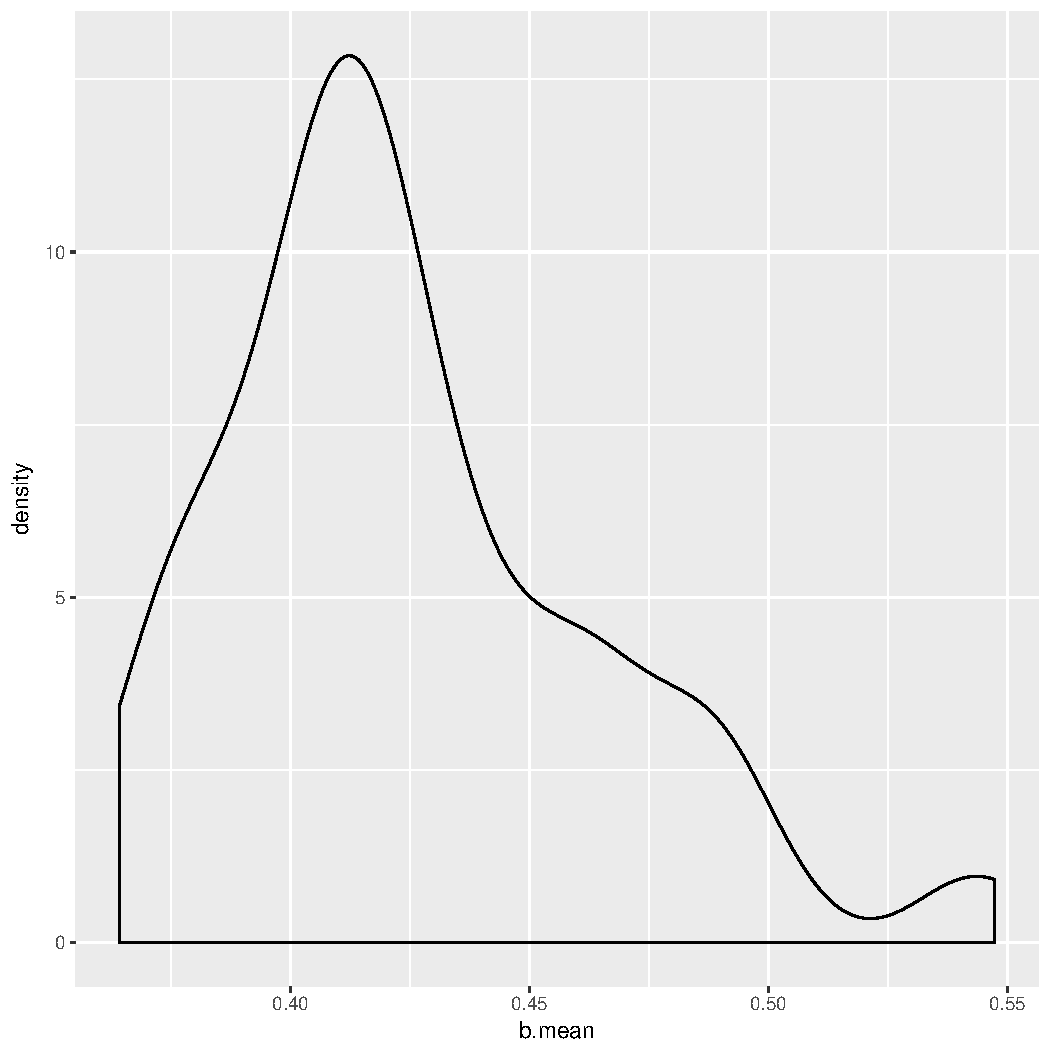
\includegraphics[width=300px]{knit_figure/figintens-1} 

}

\caption[Distribution of Vimentin intensity]{Distribution of Vimentin intensity}\label{fig:intens}
\end{figure}


\end{knitrout}


\begin{knitrout}
\definecolor{shadecolor}{rgb}{0.969, 0.969, 0.969}\color{fgcolor}\begin{kframe}
\begin{alltt}
\hlkwd{ggplot}\hlstd{(all_features,} \hlkwd{aes}\hlstd{(s.area))} \hlopt{+} \hlkwd{geom_density}\hlstd{()}
\end{alltt}
\end{kframe}\begin{figure}

{\centering 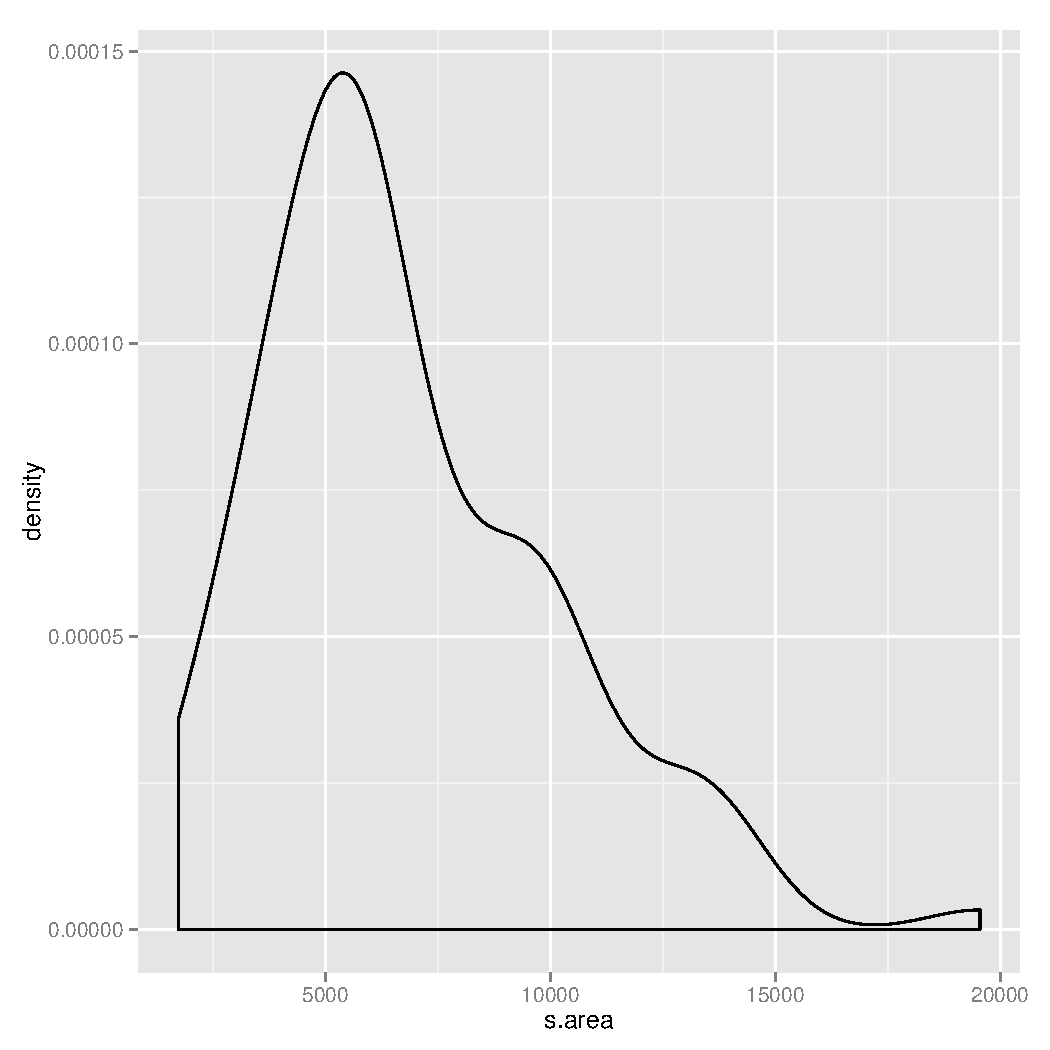
\includegraphics[width=300px]{knit_figure/figarea-1} 

}

\caption[Distribution of areas]{Distribution of areas}\label{fig:area}
\end{figure}


\end{knitrout}

\begin{knitrout}
\definecolor{shadecolor}{rgb}{0.969, 0.969, 0.969}\color{fgcolor}\begin{kframe}
\begin{alltt}
\hlkwd{ggplot}\hlstd{(all_features,} \hlkwd{aes}\hlstd{(}\hlkwc{x}\hlstd{=s.area,} \hlkwc{y}\hlstd{=b.mean))} \hlopt{+} \hlkwd{geom_point}\hlstd{()}
\end{alltt}
\end{kframe}\begin{figure}

{\centering 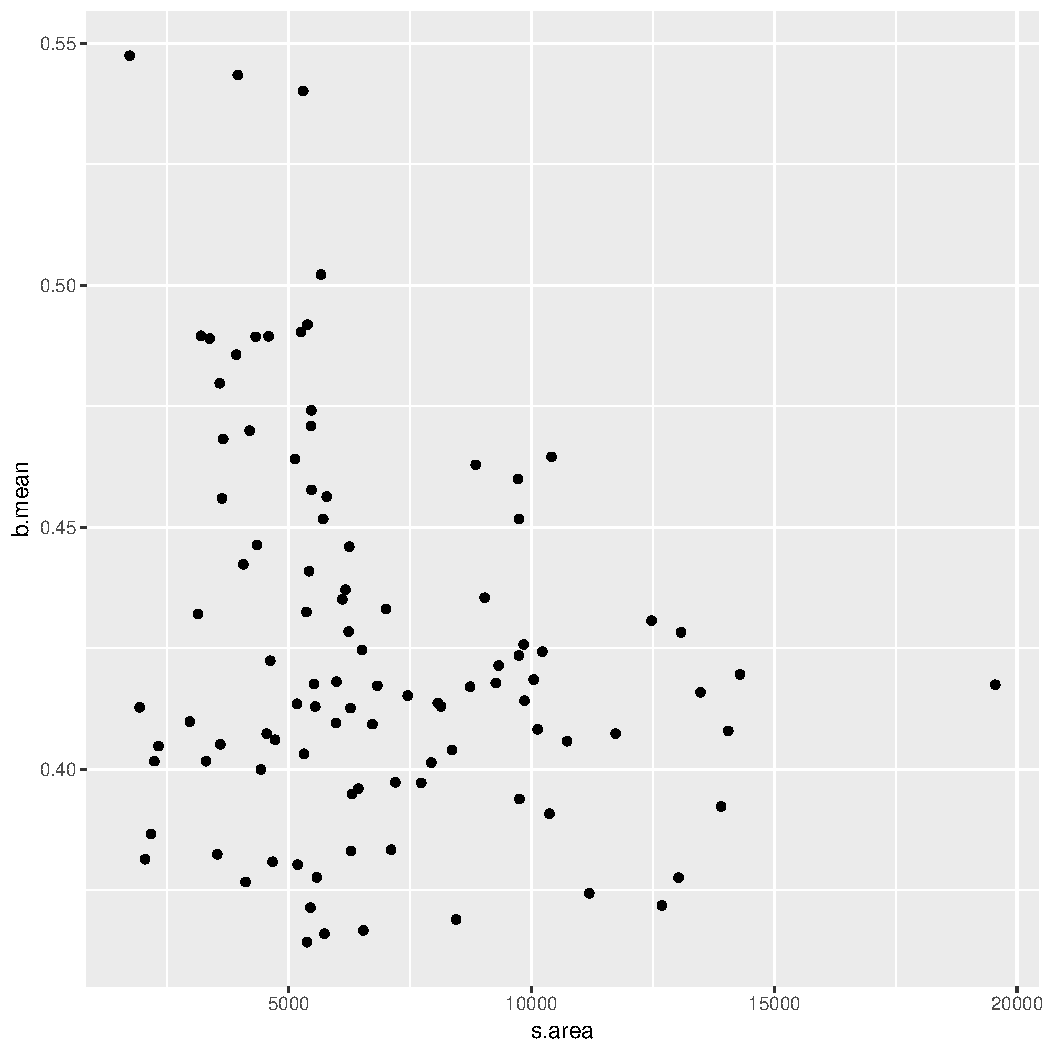
\includegraphics[width=300px]{knit_figure/figscatter-1} 

}

\caption[The area of each cell is plotted against its mean intensity]{The area of each cell is plotted against its mean intensity}\label{fig:scatter}
\end{figure}


\end{knitrout}

If we had two different populations of cells in the image, we might also be able to separate them using PCA as in Figure \ref{fig:pca}.
\begin{knitrout}
\definecolor{shadecolor}{rgb}{0.969, 0.969, 0.969}\color{fgcolor}\begin{kframe}
\begin{alltt}
\hlstd{fit} \hlkwb{<-} \hlkwd{princomp}\hlstd{(all_features,} \hlkwc{cor}\hlstd{=}\hlnum{TRUE}\hlstd{)}
\hlkwd{biplot}\hlstd{(fit)}
\end{alltt}
\end{kframe}\begin{figure}

{\centering 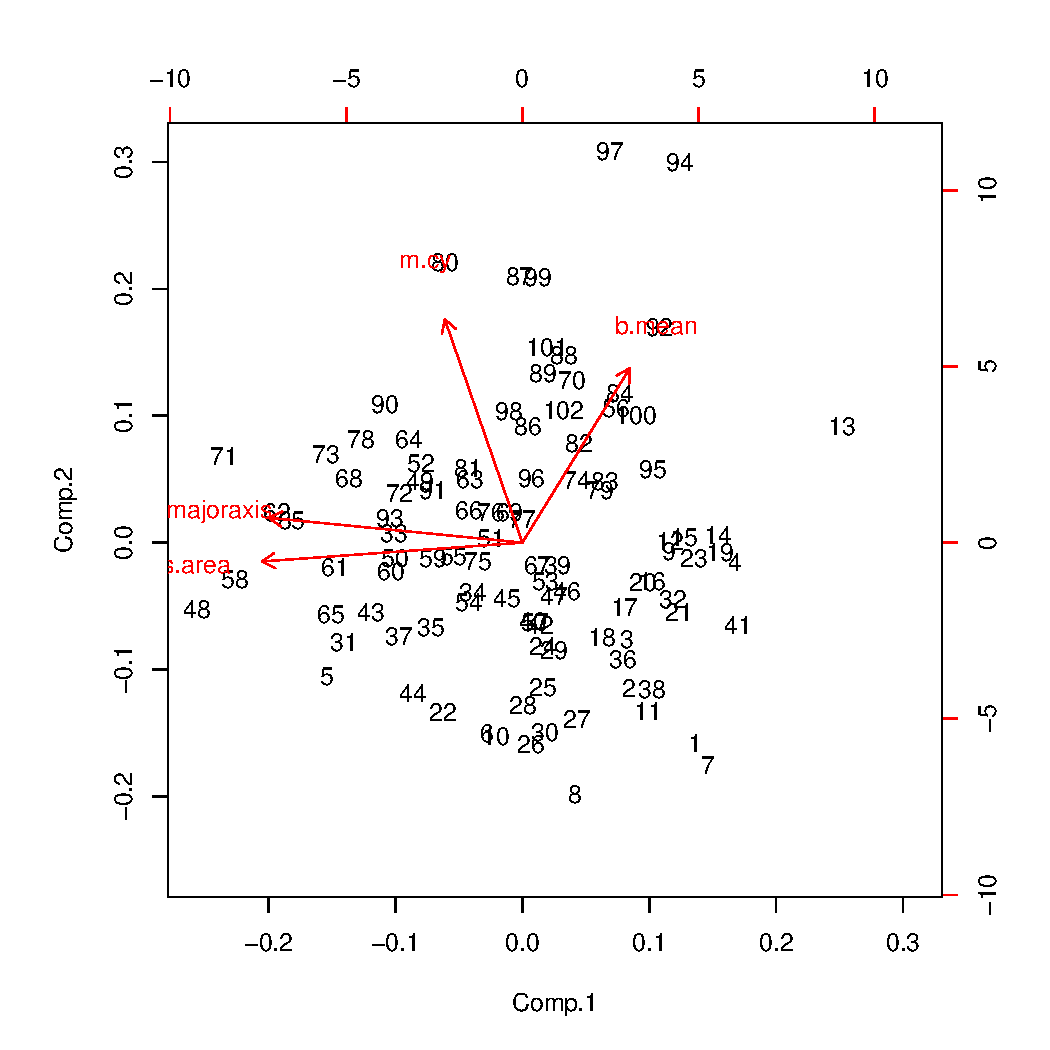
\includegraphics[width=300px]{knit_figure/figpca-1} 

}

\caption[Biplot after Principal Component Analysis]{Biplot after Principal Component Analysis}\label{fig:pca}
\end{figure}


\end{knitrout}

\end{document}
